% Options for packages loaded elsewhere
\PassOptionsToPackage{unicode}{hyperref}
\PassOptionsToPackage{hyphens}{url}
%
\documentclass[
  ignorenonframetext,
]{beamer}
\usepackage{pgfpages}
\setbeamertemplate{caption}[numbered]
\setbeamertemplate{caption label separator}{: }
\setbeamercolor{caption name}{fg=normal text.fg}
\beamertemplatenavigationsymbolsempty
% Prevent slide breaks in the middle of a paragraph
\widowpenalties 1 10000
\raggedbottom
\setbeamertemplate{part page}{
  \centering
  \begin{beamercolorbox}[sep=16pt,center]{part title}
    \usebeamerfont{part title}\insertpart\par
  \end{beamercolorbox}
}
\setbeamertemplate{section page}{
  \centering
  \begin{beamercolorbox}[sep=12pt,center]{part title}
    \usebeamerfont{section title}\insertsection\par
  \end{beamercolorbox}
}
\setbeamertemplate{subsection page}{
  \centering
  \begin{beamercolorbox}[sep=8pt,center]{part title}
    \usebeamerfont{subsection title}\insertsubsection\par
  \end{beamercolorbox}
}
\AtBeginPart{
  \frame{\partpage}
}
\AtBeginSection{
  \ifbibliography
  \else
    \frame{\sectionpage}
  \fi
}
\AtBeginSubsection{
  \frame{\subsectionpage}
}

\usepackage{amsmath,amssymb}
\usepackage{lmodern}
\usepackage{iftex}
\ifPDFTeX
  \usepackage[T1]{fontenc}
  \usepackage[utf8]{inputenc}
  \usepackage{textcomp} % provide euro and other symbols
\else % if luatex or xetex
  \usepackage{unicode-math}
  \defaultfontfeatures{Scale=MatchLowercase}
  \defaultfontfeatures[\rmfamily]{Ligatures=TeX,Scale=1}
\fi
% Use upquote if available, for straight quotes in verbatim environments
\IfFileExists{upquote.sty}{\usepackage{upquote}}{}
\IfFileExists{microtype.sty}{% use microtype if available
  \usepackage[]{microtype}
  \UseMicrotypeSet[protrusion]{basicmath} % disable protrusion for tt fonts
}{}
\makeatletter
\@ifundefined{KOMAClassName}{% if non-KOMA class
  \IfFileExists{parskip.sty}{%
    \usepackage{parskip}
  }{% else
    \setlength{\parindent}{0pt}
    \setlength{\parskip}{6pt plus 2pt minus 1pt}}
}{% if KOMA class
  \KOMAoptions{parskip=half}}
\makeatother
\usepackage{xcolor}
\newif\ifbibliography
\setlength{\emergencystretch}{3em} % prevent overfull lines
\setcounter{secnumdepth}{-\maxdimen} % remove section numbering


\providecommand{\tightlist}{%
  \setlength{\itemsep}{0pt}\setlength{\parskip}{0pt}}\usepackage{longtable,booktabs,array}
\usepackage{calc} % for calculating minipage widths
\usepackage{caption}
% Make caption package work with longtable
\makeatletter
\def\fnum@table{\tablename~\thetable}
\makeatother
\usepackage{graphicx}
\makeatletter
\def\maxwidth{\ifdim\Gin@nat@width>\linewidth\linewidth\else\Gin@nat@width\fi}
\def\maxheight{\ifdim\Gin@nat@height>\textheight\textheight\else\Gin@nat@height\fi}
\makeatother
% Scale images if necessary, so that they will not overflow the page
% margins by default, and it is still possible to overwrite the defaults
% using explicit options in \includegraphics[width, height, ...]{}
\setkeys{Gin}{width=\maxwidth,height=\maxheight,keepaspectratio}
% Set default figure placement to htbp
\makeatletter
\def\fps@figure{htbp}
\makeatother

\makeatletter
\makeatother
\makeatletter
\makeatother
\makeatletter
\@ifpackageloaded{caption}{}{\usepackage{caption}}
\AtBeginDocument{%
\ifdefined\contentsname
  \renewcommand*\contentsname{Table of contents}
\else
  \newcommand\contentsname{Table of contents}
\fi
\ifdefined\listfigurename
  \renewcommand*\listfigurename{List of Figures}
\else
  \newcommand\listfigurename{List of Figures}
\fi
\ifdefined\listtablename
  \renewcommand*\listtablename{List of Tables}
\else
  \newcommand\listtablename{List of Tables}
\fi
\ifdefined\figurename
  \renewcommand*\figurename{Figure}
\else
  \newcommand\figurename{Figure}
\fi
\ifdefined\tablename
  \renewcommand*\tablename{Table}
\else
  \newcommand\tablename{Table}
\fi
}
\@ifpackageloaded{float}{}{\usepackage{float}}
\floatstyle{ruled}
\@ifundefined{c@chapter}{\newfloat{codelisting}{h}{lop}}{\newfloat{codelisting}{h}{lop}[chapter]}
\floatname{codelisting}{Listing}
\newcommand*\listoflistings{\listof{codelisting}{List of Listings}}
\makeatother
\makeatletter
\@ifpackageloaded{caption}{}{\usepackage{caption}}
\@ifpackageloaded{subcaption}{}{\usepackage{subcaption}}
\makeatother
\makeatletter
\@ifpackageloaded{tcolorbox}{}{\usepackage[many]{tcolorbox}}
\makeatother
\makeatletter
\@ifundefined{shadecolor}{\definecolor{shadecolor}{rgb}{.97, .97, .97}}
\makeatother
\makeatletter
\makeatother
\ifLuaTeX
  \usepackage{selnolig}  % disable illegal ligatures
\fi
\IfFileExists{bookmark.sty}{\usepackage{bookmark}}{\usepackage{hyperref}}
\IfFileExists{xurl.sty}{\usepackage{xurl}}{} % add URL line breaks if available
\urlstyle{same} % disable monospaced font for URLs
\hypersetup{
  pdftitle={Eppur si muove},
  hidelinks,
  pdfcreator={LaTeX via pandoc}}

\title{Eppur si muove}
\subtitle{El efecto de las aspersiones aéreas con glifosato en el
desplazamiento forzado en Colombia}
\author{}
\date{}

\begin{document}
\frame{\titlepage}
\ifdefined\Shaded\renewenvironment{Shaded}{\begin{tcolorbox}[boxrule=0pt, enhanced, breakable, interior hidden, borderline west={3pt}{0pt}{shadecolor}, sharp corners, frame hidden]}{\end{tcolorbox}}\fi

\hypertarget{introducciuxf3n} de la
  población actual.\\
\item
  Aunque hay motivos relacionados con la violencia, las causas pueden ir
  más allá.\\
\item
  En el contexto de conflicto armado y guerra contra las drogas, se creó
  \textbf{el Plan Colombia}.\\
\item
  Las aspersiones, el programa principal del Plan Colombia, tuvieron
  efectos negativos sobre la población.
\end{itemize}
\end{frame}

\begin{frame}{Motivación}
\protect\hypertarget{motivaciuxf3n-1}{}
\hfill\break
\hfill\break

``El desplazamiento que se tuvo, que se vio en ese tiempo, fue bastante
masivo. La gente salió y el territorio quedó prácticamente solo y la
atención a las comunidades fue mínima por parte del gobierno. Como digo,
no había un plan de contingencia para atender a las personas desplazadas
por las fumigaciones; no lo hubo, ni lo hay'' (Yonda, 2021)
\end{frame}

\hypertarget{pregunta-de-investigaciuxf3n}{%
\section{Pregunta de investigación}\label{pregunta-de-investigaciuxf3n}}

\begin{frame}{Pregunta de investigación}
\protect\hypertarget{pregunta-de-investigaciuxf3n-1}{}
\hfill\break
\hfill\break
\hfill\break

\textbf{¿Cuál es la magnitud del efecto de las aspersiones áereas con
glifosato (PECIG) sobre el desplazamiento?}
\end{frame}

\begin{frame}{Principales hallazgos}
\protect\hypertarget{principales-hallazgos}{}
\hfill\break

\begin{itemize}
\item
  Ante un aumento de un punto porcentual en la intesidad de aspersión
  implica un aumento de \textbf{3.73 puntos porcentuales} en la tasa de
  desplazamiento agregada en el tiempo.

  \begin{itemize}
  \tightlist
  \item
    En el mes inmediatamente después de la aspersión el aumento es de
    \textbf{1,28 puntos porcentuales}.
  \item
    En el segundo mes el aumento es de \textbf{1,46 puntos
    porcentuales}.
  \item
    En el tercer mes el aumento es de \textbf{1.3 puntos porcentuales}.
  \end{itemize}
\item
  \textbf{La reiteración de la aspersión intensifica} los niveles de
  desplazamiento producidos por la aspersión.
\item
  Existen efectos heterogéneos en la relación de acuerdo al
  \textbf{volumen de cultivos de coca}.
\end{itemize}
\end{frame}

\hypertarget{metodologuxeda}{%
\section{Metodología}\label{metodologuxeda}}

\begin{frame}{Estrategia empírica}
\protect\hypertarget{estrategia-empuxedrica}{}
\end{frame}

\hypertarget{resultados}{%
\section{Resultados}\label{resultados}}

\begin{frame}{Resultados}
\protect\hypertarget{resultados-1}{}
\begin{block}{Gráfica}
\protect\hypertarget{gruxe1fica}{}
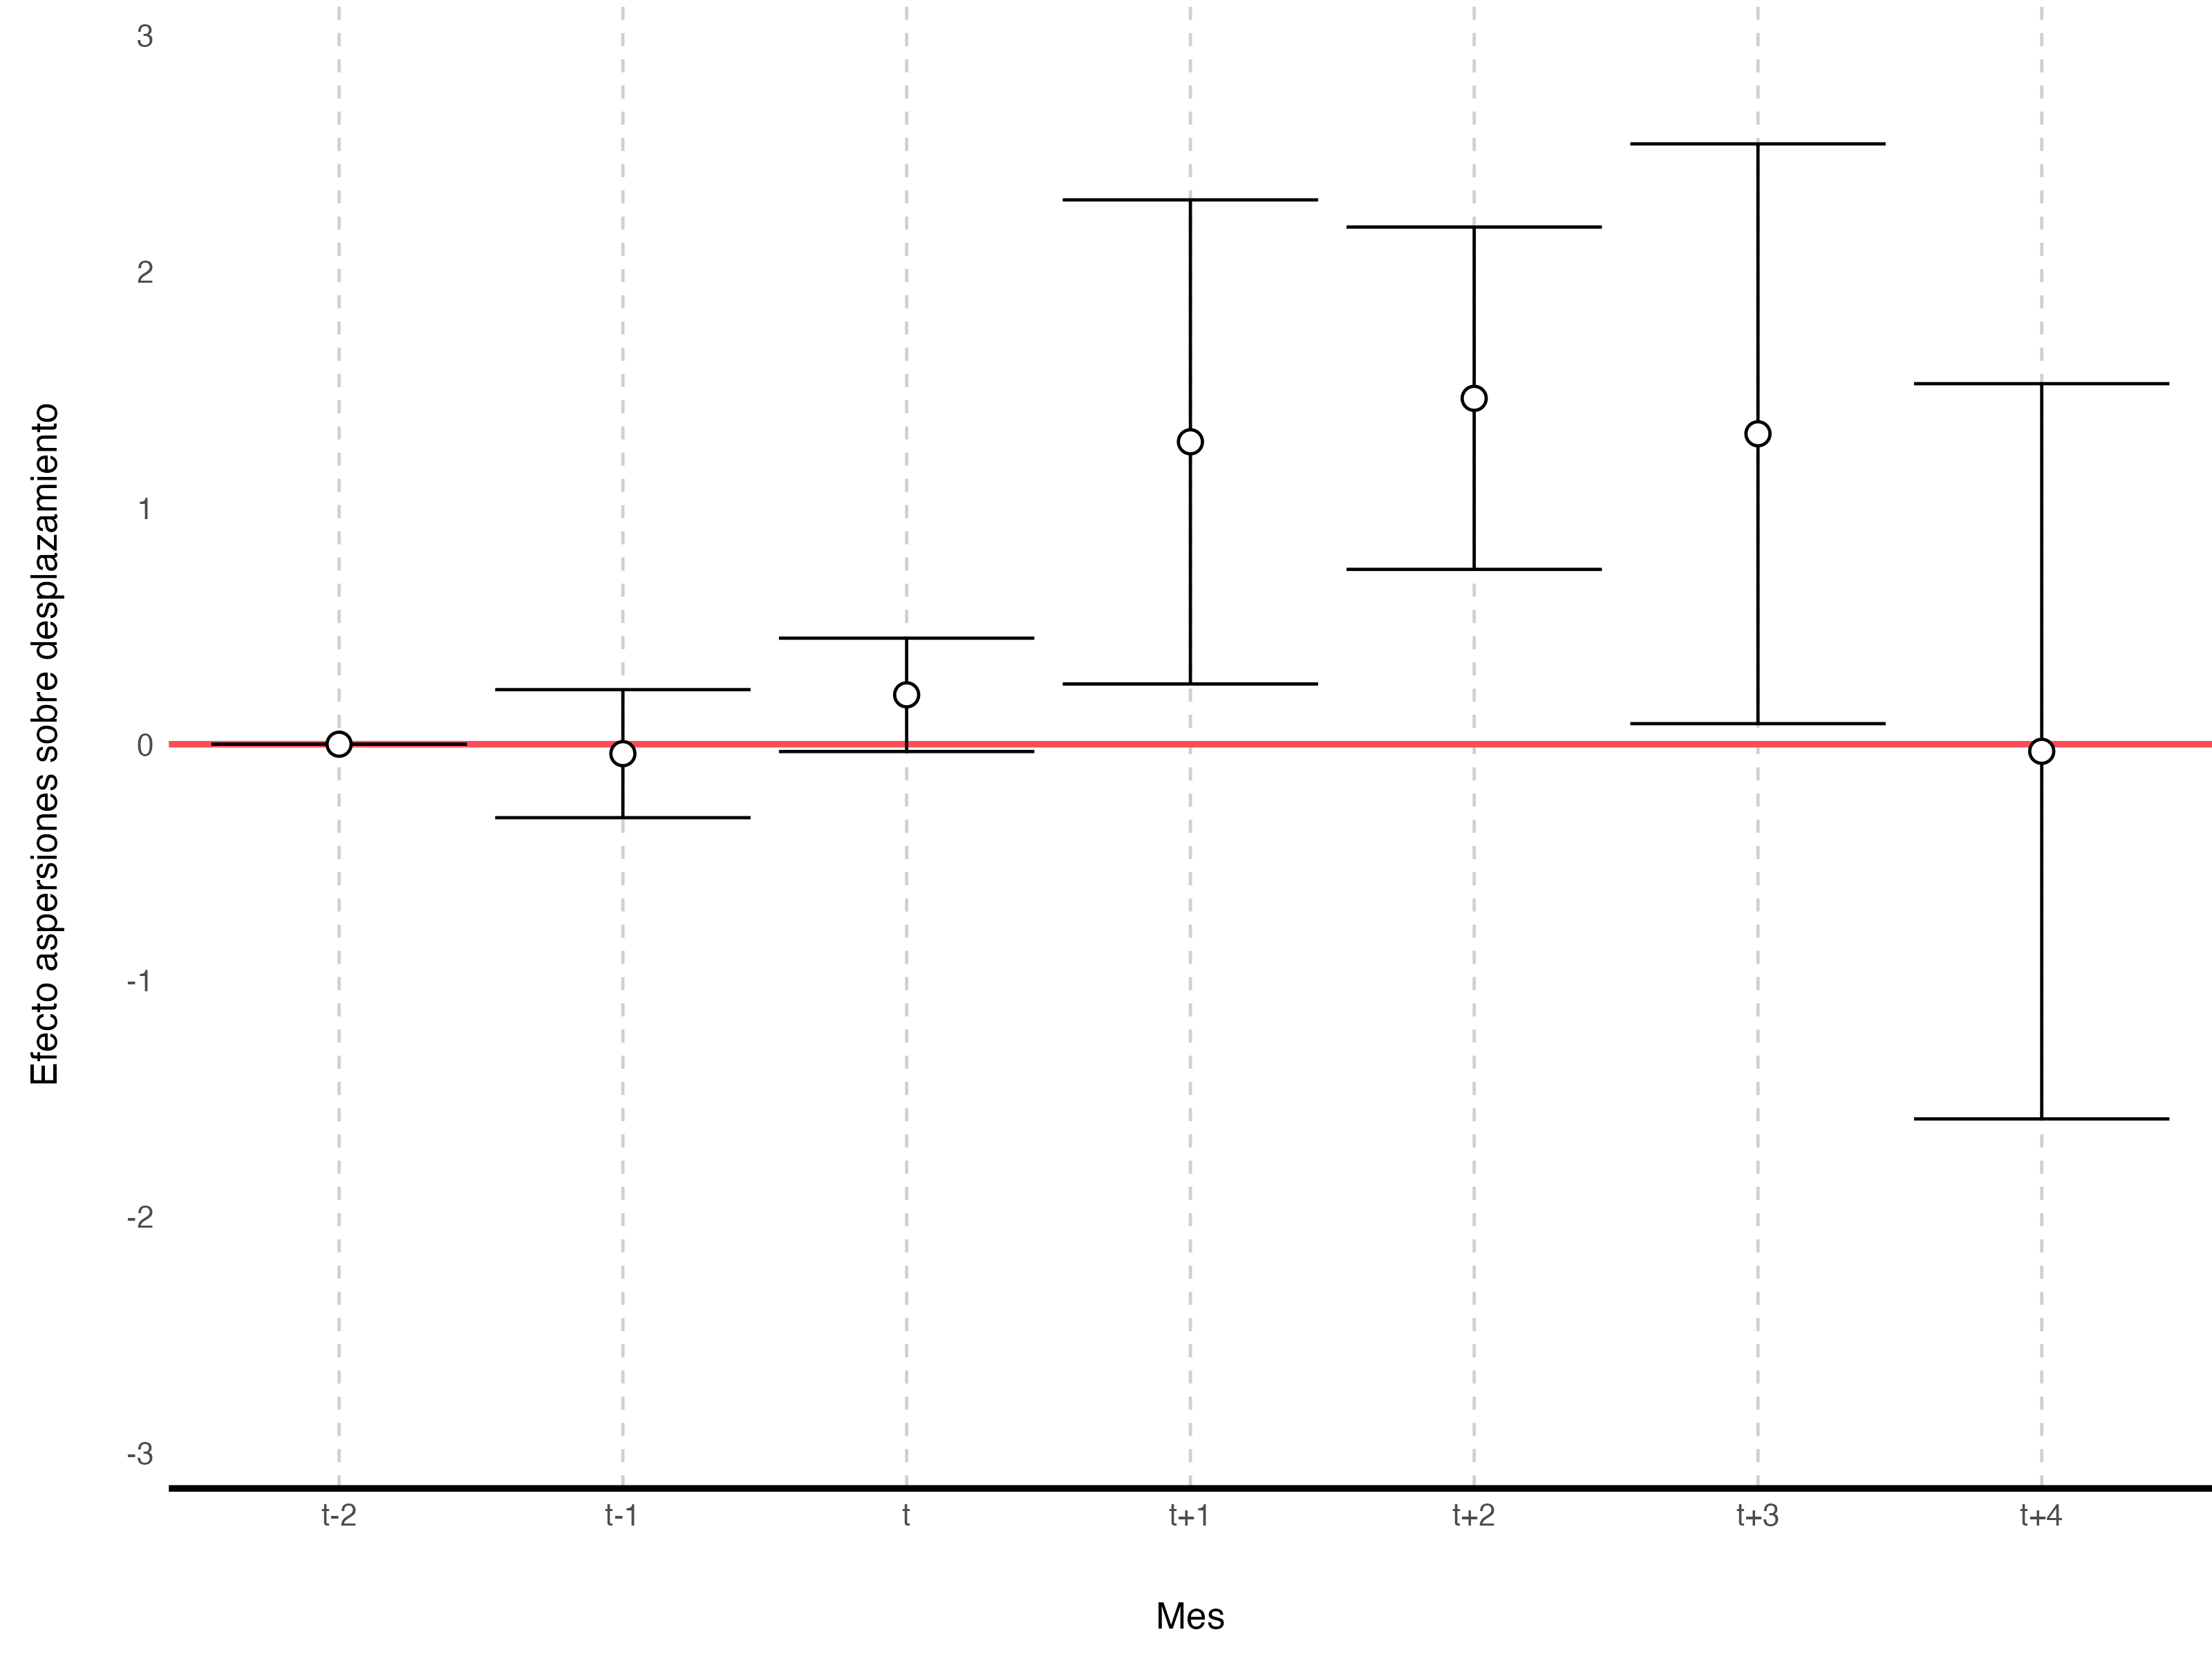
\includegraphics[width=0.5\textwidth,height=\textheight]{media/DinamicEffectsNorm.png}
\end{block}

\begin{block}{Tabla}
\protect\hypertarget{tabla}{}
\begin{table}[!htbp] \centering 
  \caption{Relación entre aspersiones aéreas y el desplazamiento en meses posteriores} 
  \label{} 
\begin{threeparttable}
\begin{tabular}{@{\extracolsep{5pt}}lD{,}{,}{-3} D{,}{,}{-3} D{,}{,}{-3} } 
\\[-1.8ex]\hline 
\hline \\[-1.8ex] 
 & \multicolumn{3}{c}{Variable dependiente: Desplazamiento Forzado} \\ 
\cline{2-4} 
\\[-1.8ex] & \multicolumn{1}{c}{(t + 1)} & \multicolumn{1}{c}{(t + 2)} & \multicolumn{1}{c}{(t + 3)}\\ 
\hline \\[-1.8ex] 
 Aspersiones aéreas & 1,280^{**} & 1,464^{***} & 1,314^{*} \\ 
  & (0,623) & (0,440) & (0,746) \\ 
  & & & \\ 
\hline \\[-1.8ex] 
Efectos Fijos & Si & Si & Si \\ 
Controles & Si & Si & Si \\ 
Observaciones & \multicolumn{1}{c}{10,246} & \multicolumn{1}{c}{10,058} & \multicolumn{1}{c}{9,868} \\ 
R$^{2}$ & \multicolumn{1}{c}{0,001} & \multicolumn{1}{c}{0,0001} & \multicolumn{1}{c}{0,00001} \\ 
\hline 
\end{tabular} 
\begin{tablenotes}[flushleft] 
        \tiny % el tamaño de la fuente de la nota
        \item Nota: Los errores fueron clusterizado a nivel municipal. Los valores dentro de los parentesis representan la desviación estandar. Paralelamente se aplicaron efectos fijos por municipio, año-mes y núcleo. Las variables de control asociadas a la violencia se tomaron en tasas por 100 habitantes, estas son: desaparición forzada, reclutamiento de menores, minas, combates y despojo. Las variables de control geograficas son: choques de viento, indice de vegetación y niveles de lluvia. La variable de control asociada al desarrollo economico es la intensidad de luminosidad del municipio. Además, los niveles de signifancia se ven representados de la siguiente manera: $^{*}$p$<$0,1; $^{**}$p$<$0,05; $^{***}$p$<$0,01  
\end{tablenotes}
\end{threeparttable}
\end{table}
\end{block}
\end{frame}

\begin{frame}{Mecanismos}
\protect\hypertarget{mecanismos}{}
\end{frame}

\hypertarget{conclusiones}{%
\section{Conclusiones}\label{conclusiones}}



\end{document}
